\documentclass[conference]{IEEEtran}
\usepackage{cite}
\usepackage{amsmath,amssymb,amsfonts}
\usepackage{algorithmic}
\usepackage{graphicx}
\usepackage{textcomp}
\usepackage{xcolor}
\def\BibTeX{{\rm B\kern-.05em{\sc i\kern-.025em b}\kern-.08em
    T\kern-.1667em\lower.7ex\hbox{E}\kern-.125emX}}
\begin{document}
\title{Comparison Among Automatic Exploration Tools for Android Applications}

\author{\IEEEauthorblockN{Michael Osorio-Riaño}
\IEEEauthorblockA{\textit{Department of Systems and Computing Engineering } \\
\textit{University of Los Andes}\\
Bogotá, Colombia\\
ms.osorio@uniandes.edu.co}
\textit{Advised by: Mario Linares-Vásquez}\\
\textit{m.linaresv@uniandes.edu.co}\\
\textit{Assistant Professor at University of Los Andes}
}

\maketitle

\begin{IEEEkeywords}
Android, Móvil, Pruebas, Exploración Automática,Ingeniería de Software empírica
\end{IEEEkeywords}

\section{motivación}
La gran cantidad de aplicaciones móviles que se han generado a lo largo de los últimos diez años, ha llevado a que grandes investigadores desarrollen herramientas y patrones para la mejora de la calidad de ese tipo de productos de software, como por ejemplo, las herramientas de exploración automática de aplicaciones móviles. Dada la cantidad de herramientas de exploración automática existentes y el surgimiento de otras de ese mismo tipo cada día, se hace indispensable pensar en cuál de ellas brinda mejores características que las demás, a ciertos proyectos y cuales, por el contrario, añaden limitaciones o simplemente no brinda las mismas características que otros. Es por lo anterior que en este documento se propone realizar una investigación que se basará en un estudió empírico, discutirá por lo menos 3 de las mencionadas herramientas de exploración automática y las comparará. Destacando las cualidades y defectos de cada una. Además, realizará énfasis en la comparación de RIP en su versión Java contra RIP en su versión Kotlin.
\section{Trabajos relacionados y estado del arte}
Existen herramientas destinadas únicamente a la exploración de aplicaciones móviles como la oficial de Android (Android monkey) \cite{b1}, la cuál realiza su exploración con interacciones aleatorias a lo largo de la pantalla y de la aplicación. Por otro lado, existen estudios y herramientas como Android testing framework \cite{b2}, Mobicomonkey \cite{b3}, y algunas otras \cite{b4, b5, b6}, las cuales proponen diferentes metodologías de exploración, combinando diferentes técnicas de comparación y priorización de interacciones, además de buscar optimizar este proceso con la aplicación de estrategias para reducir la cantidad de combinaciones en pruebas exhaustivas. Finalmente, se descubrió BBoxTester \cite{b7} el cuál es un framework que generar medidas de cobertura de código para herramientas de pruebas automáticas, permitiendo así la elección de herramientas de forma objetiva con base en las medidas generadas.

Las publicaciones encontradas anteriormente tratan la exploración automática pero no se enfocan en la comparación de las herramientas existentes. Por el contrario, todas ellas proponen una nueva herramienta con diferentes estrategias de exploración y priorización. La publicación que más se acerca al trabajo que se plantea en este documento es \cite{b7}, gracias a la generación de métricas que permiten comparar objetivamente herramientas de exploración y de pruebas automáticas de aplicaciones móviles Android.

\section{Objetivos Generales y Específicos}
\begin{itemize}
	\item Objetivo General:
		Identificar y comparar herramientas de exploración sistemática de aplicaciones móviles Android encontrando sus características, beneficios y limitaciones
	\item Específicos:
		\begin{enumerate}
			\item Identificar herramientas de exploración automática existentes diferentes a RIP
			\item Comparar las herramientas encontradas, incluyendo la versión Kotlin de RIP, destacando los puntos positivos y negativos de cada herramienta
		\end{enumerate}
\end{itemize}

\section{Actividades}
	\begin{enumerate}
		\item Fase 1: 
		\begin{enumerate}
			\item Búsqueda de trabajos relacionados
			\item Lectura de los trabajos encontrados
		\end{enumerate}
		\item Fase 2: Implementación
		\begin{enumerate}
			\item Replicar las funcionalidades de RIP Base usando el lenguaje de programación Kotlin
			\item Replicar las funcionalidades de RIPRR usando el lenguaje de programación Kotlin
		\end{enumerate}
		\item Fase 3: Experimentación, generación y recolección de datos
		\begin{enumerate}
			\item Búsqueda del conjunto de pruebas
			\item Realización de pruebas entre las versiones de Java y Kotlin de RIP Base y RIPRR. 
			\item Recolección de métricas de desempeño de ambas versiones de RIP*
			\item Registro de los datos y estadísticas de las dos versiones de RIP*: líneas de código, tamaño de los proyectos, tamaño de los ejecutables, etc.\
			\item Ejecución de las herramientas encontradas sobre el mismo conjunto de datos
			\item Recolección de métricas de desempeño de las herramientas encontradas diferentes a RIP*
		\end{enumerate}
		\item Fase 4: Desarrollo de entregables
		\begin{enumerate}
			\item Realizar la comparación y el reporte del consumo de recursos entre las dos versiones de RIP* y las demás herramientas
			\item Realizar la comparación y el reporte del tiempo de ejecución entre las dos versiones de RIP* y las demás herramientas
			\item Realizar la comparación y análisis de estadísticas de las dos versiones de RIP* a nivel de código y de proyecto
			\item Realizar el reporte de las diferencias en la exploración que hayan sido encontradas: Número de estados, número de transiciones realizadas, etc. entre las dos versiones de RIP* y las demás herramientas
		\end{enumerate}
	\end{enumerate}
La realización de estas actividades están separadas a lo largo de 4 meses. La distribución detallada de cada fase a lo largo del tiempo está explicada en la figura 1.

\section{Resultados Esperados}
Se espera generar la cantidad adecuada de datos que permitan encontrar las estadísticas y resultados necesarios para la comparación objetiva de las diferentes herramientas que serán encontradas y desarrolladas en la fase 1 y 2, respectivamente, y probadas en la fase 3.

Dada la posibilidad de no encontrar una herramienta mejor que otra, se desea poder listar las ventajas que tiene el uso de alguna de estas herramientas en un contexto específico, y los perjuicios o desventajas de usarla en otro contexto, lo que permitiría mejorar la elección de la herramienta que se utilizará en las pruebas de una aplicación móvil Android, basándose en criterios objetivos que le posibilita a los desarrolladores sacar el mejor provecho y mejorar en mayor medida la calidad de sus productos.

Los resultados se resumen como sigue: 
\begin{enumerate}
	\item Versión Kotlin de la herramienta RIPBase
	\item Versión Kotlin de la herramienta RIPRR
	\item Texto que abarca: 
		\begin{enumerate}
			\item Cuadro comparativo del desempeño de ambas versiones de RIP* y las demás herramientas que sean encontradas y probadas
			\item Cuadro comparativo a nivel de código y proyecto entre las versiones de RIP* Java y Kotlin.
			\item Análisis de resultados del desempeño de las herramientas comparadas
			\item Conclusiones relevantes que ayuden a la selección objetiva de herramientas de exploración automática, con el fin de favorecer el proceso de pruebas de aplicaciones móviles Android
		\end{enumerate}
\end{enumerate}

\begin{figure}[h]
	\includegraphics[angle = 90,width=0.5\textwidth, height =0.83\textheight]			{cronograma}
	\caption{Cronograma de actividades}
	\label{fig}
\end{figure}

\begin{thebibliography}{00}
\bibitem{b1} Android monkey,

\section{Study}
\label{sec:study}
In order to measure the method coverage reached by an exploration tool in one application, there is the need to know how many methods there are in the application and how many methods were called during the exploration. To achieve that, the application developers could count the number of methods in their project and write log lines at the beginning of every method. After that, they will need to compile, run the exploration tool against their application, measure the number of methods that were called during the exploration and compute statistics.

With that in mind, this study consists of nearly the same stages, i. instrumentation, ii. exploration, iii. coverage analysis, iv. summarize, and v. compute statistics. The stages ii. and iii. were repeated 10 times for every application that was selected, that leaded to the iv. stage.

The different stages were completed as follow:

Stage i: The applications' instrumentation was made by using InstruAPK. It is an instrumentation tool developed mainly for this study. This tool uses APKTool, a known Java application that allows inverse engineering in Android apps, allowing applications' instrumentation without the need of recompiling their source code. APKTool decodes the apk and the result is the smali representation of the app source code, These smali files are analysed in order to find all the methods to be instrumented and then, the log code is injected at the very beginning of each method. Its important to notice that no external libraries methods are instrumented. InstruAPK only search for methods following the android project structure that uses the application package name to store the application source code.

Stage ii: The exploration was made by four different automatic exploration tools. two from the industry and two from the academic side. The first tool was Firebase Test Lab. it was selected for being widely used in industry and for also being a Google product. The second one, Monkey, was selected for being the most basic one and because it is also included in the SDK for developing Android Apps. The third one, Droidbot, was selected from the academic side. Droidbot has been a point of study for many researches. Many others tools have based their functionality on this tool. The last one is RIP, this tool was selected for being of special interest for us. It is our own exploration tool and is is currently an active project inside the Software Design Lab at University of Los Andes. 

Every tool was executed ten times per application, and every execution with a maximum time of 30 minutes. Some tools ended its exploration before the max time. 
The number of executions and the maximum time were arbitrary decisions that were made because of time limitations for the study. Although, during the study was notice that most of the tools ended the exploration or reached their maximum coverage within the first 15 minutes. Which means that the maximum time for exploration was more than enough in almost all cases. 
 
stage iii: The coverage measurement was made by CoverageAnalyzer. It is a Java Application created mainly for this study. This tool analyses the resulting logcat of an Android phone, when executing an application that was instrumented by InstruAPK. It extracts different data such as, number of methods called, number of  methods never called, number of error traces of the application being analysed, most called methods, less called methods, as well as the time stamp of all calls of every method. It is important to notice that the possibility of extracting all those information is because InstruAPK provides it.

stage iv: Due to the multiple executions of every APK per tool, it is important to summarize de data. The final report contains the total number of unique methods called during all ten executions, reporting only the first time they were called.
The exploration reports are analysed and filtered as well.

stage v: This is the final stage of the study that involves, understanding data, computing statistics, creating graphs, extract insights and conclusions. 

Besides that, for this study, a set of 11 applications was used. This set is a subset of a set of open source applications utilised inside The Software Design Lab research group for other studies and tests, including RIP. Every APK in the subset should be successfully instrumented by InstruAPK, it should compile without any problem after instrumentation and it should be launch in an emulator without any issue after instrumentation.

\begin{figure}[h]
	\centering
	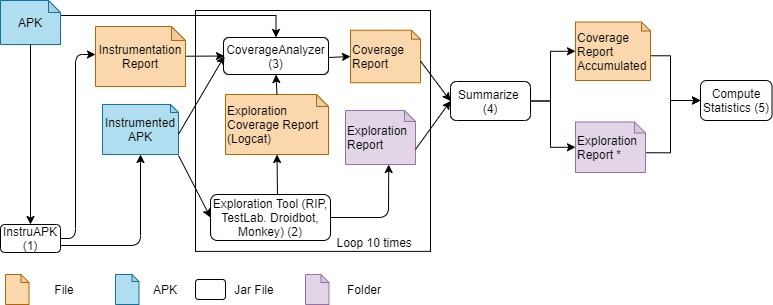
\includegraphics[width=0.5\textwidth]{img/workflow.jpg}
	\vspace{-0.5cm}
	\caption{Complete Study Workflow}
	\label{procesoTests}
\end{figure} 


http://developer.android.com/guide/developing/tools/monkey.html.
\bibitem{b2}Android testing framework,

http://developer.android.com/guide/topics/testing/index.html.
\bibitem {b3} Amit Seal Ami, Md. Mehedi Hasan, Md. Rayhanur Rahman, and Kazi Sakib. 2018. Mobicomonkey: context testing of Android apps. In Proceedings of the 5th International Conference on Mobile Software Engineering and Systems (MOBILESoft '18). ACM, New York, NY, USA, 76-79.
\bibitem{b4} Young-Min Baek and Doo-Hwan Bae. 2016. Automated model-based Android GUI testing using multi-level GUI comparison criteria. In Proceedings of the 31st IEEE/ACM International Conference on Automated Software Engineering (ASE 2016). ACM, New York, NY, USA, 238-249.
\bibitem{b5} Ting Su, Guozhu Meng, Yuting Chen, Ke Wu, Weiming Yang, Yao Yao, Geguang Pu, Yang Liu, and Zhendong Su. 2017. Guided, stochastic model-based GUI testing of Android apps. In Proceedings of the 2017 11th Joint Meeting on Foundations of Software Engineering (ESEC/FSE 2017). ACM, New York, NY, USA, 245-256.
\bibitem{b6} Nariman Mirzaei, Joshua Garcia, Hamid Bagheri, Alireza Sadeghi, and Sam Malek. 2016. Reducing combinatorics in GUI testing of android applications. In Proceedings of the 38th International Conference on Software Engineering (ICSE '16). ACM, New York, NY, USA, 559-570.
\bibitem {b7} Y. Zhauniarovich, A. Philippov, O. Gadyatskaya, B. Crispo and F. Massacci, "Towards Black Box Testing of Android Apps," 2015 10th International Conference on Availability, Reliability and Security, Toulouse, 2015, pp. 501-510.
\end{thebibliography}


\end{document}